\begin{figure*}
\centering
\begin{multicols}{2}
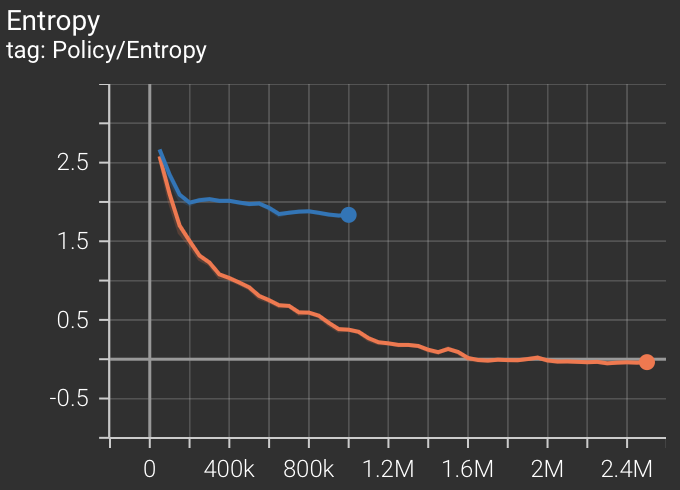
\includegraphics[width=0.99\columnwidth]{Chapter3/Epsilon/epsi_Entropy.png}\par
\caption{Higher epsilon value of 0.3 (orange) achieves lower entropy than lower epsilon value of 0.1 (blue).}
\label{fig:eps_entropy}

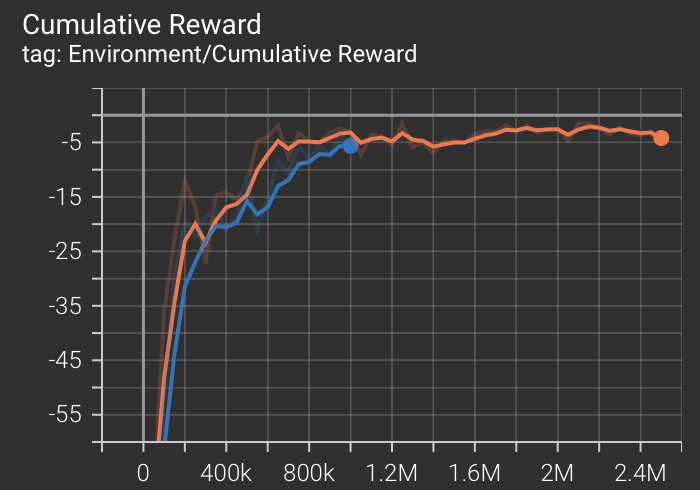
\includegraphics[width=0.99\linewidth]{Chapter3/Epsilon/eps_cum.png}\par
\caption{Higher epsilon value of 0.3 (orange) achieves slightly higher rewards than lower epsilon value of 0.1 (blue).}
\label{fig:eps_cumrewards}

\end{multicols}
\end{figure*}


\begin{figure*}
\centering
\begin{multicols}{2}
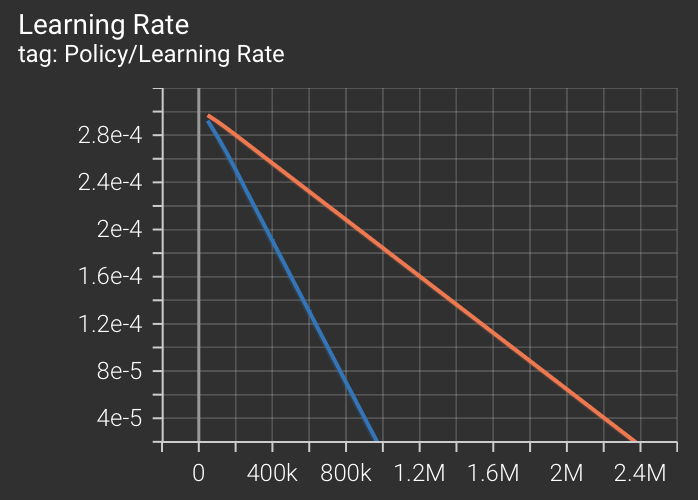
\includegraphics[width=0.99\columnwidth]{Chapter3/Epsilon/Learning_rate.png}\par
\caption{Higher epsilon value of 0.3 (orange) reduces learning rate slower than lower epsilon value of 0.1 (blue).}
\label{fig:learning_rate}

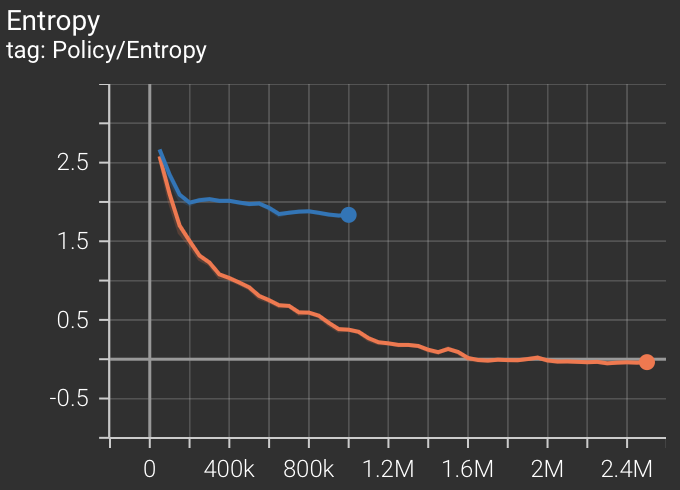
\includegraphics[width=0.99\linewidth]{Chapter3/Epsilon/epsi_Entropy.png}\par
\caption{Higher epsilon value of 0.3 (orange) is reduced over time to help stabilize training when time horizons shortens.}
\label{fig:eps}

\end{multicols}
\end{figure*}
